\documentclass[aspectratio=169]{beamer}
\beamertemplatenavigationsymbolsempty
\usecolortheme{beaver}
\setbeamertemplate{blocks}[rounded=true, shadow=true]
\setbeamertemplate{footline}[page number]
%
\usepackage[utf8]{inputenc}
\usepackage[english,russian]{babel}
\usepackage{amssymb,amsfonts,amsmath,mathtext}
\usepackage{subfig}
\usepackage[all]{xy} % xy package for diagrams
\usepackage{array}
\usepackage{multicol}% many columns in slide
\usepackage{hyperref}% urls
\usepackage{hhline}%tables
% Your figures are here:
\graphicspath{ {fig/} {../fig/} }
\newtheorem{theorem_rus}{Теорема}
\newtheorem{lemma_rus}{Лемма}
\setbeamertemplate{theorems}[numbered]
\setbeamertemplate{caption}[numbered]

%----------------------------------------------------------------------------------------------------------
\title[\hbox to 56mm{Мат. модель эффекта обратной связки с системах ИИ}]{Математическая модель эффекта обратной связи в системах искусственного интеллекта}
\author[А.\,С.~Веприков]{Андрей Сергеевич Веприков\\
\small Научный руководитель: д.ф.-м.н. А.\,С.~Хританков}
\institute{Кафедра интеллектуальных систем ФПМИ МФТИ\\
Специализация: Интеллектуальный анализ данных\\
Направление: 03.04.01 Прикладные математика и физика}
\date{2024}

%----------------------------------------------------------------------------------------------------------
\begin{document}
%----------------------------------------------------------------------------------------------------------
\begin{frame}
\thispagestyle{empty}
\maketitle
\end{frame}
%-----------------------------------------------------------------------------------------------------
\begin{frame}{Цель исследования}
    В данной работе решается задача математического моделирования систем с адаптивным управлением. Системе с ИИ ставится в соответствие дискретная динамическая система, по поведению которой можно судить об исходном объекте.
    \vspace{-1mm}
    \begin{columns}[c]
    \column{0.6\textwidth}
    \begin{figure}
        \centering
        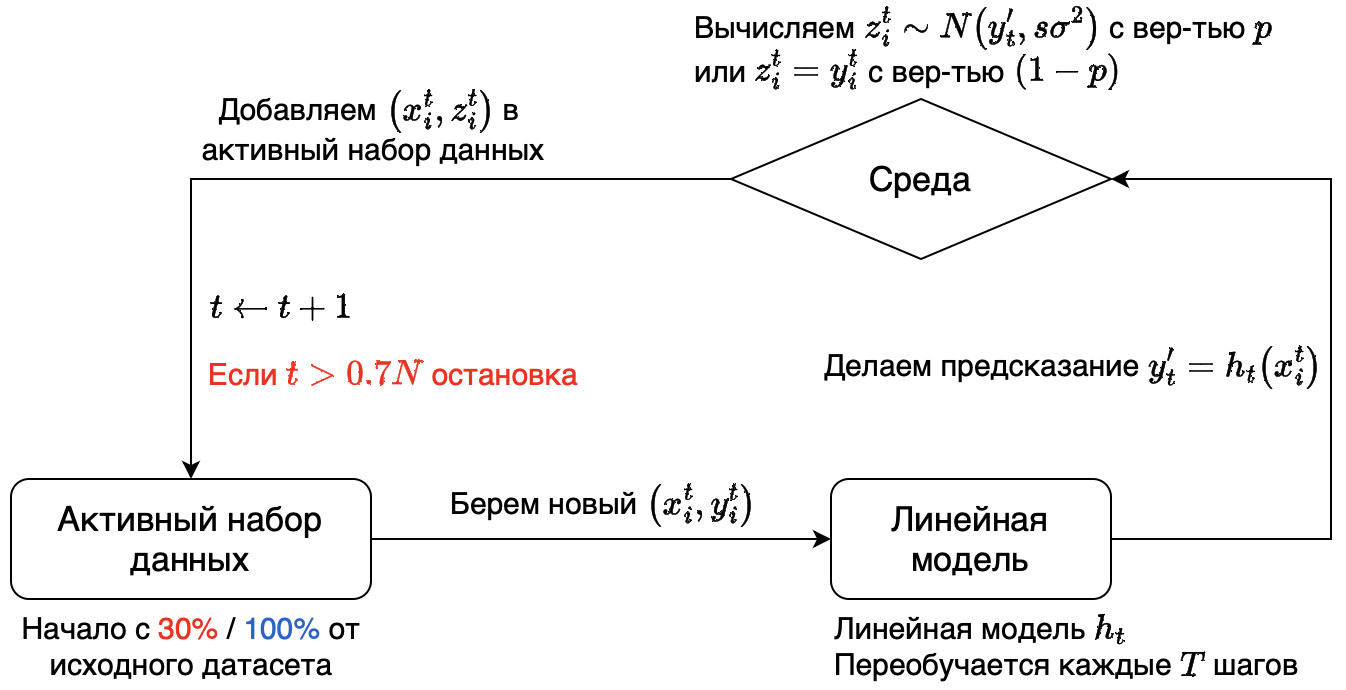
\includegraphics[width=0.99\textwidth]{fig/Experiment_setups.png}
        \vspace{-2mm}
        \caption{Две постановки эксперимента. \color{red}Скользящее окно \color{black}и \color{blue}обновление выборки.}
        \label{exp}
    \end{figure}
    \column{0.4\textwidth}
        Примеры процессов многократного машинного обучения:
    \begin{enumerate}
        \item Эффекты петель обратной связи (feedback loop) 
        \item Усиление ошибок (error amplification) 
        \item Пузыри фильтров (filter bubbles) и эхо-камеры (echo chambers) 
    \end{enumerate}
    \end{columns}
    
\end{frame}

%----------------------------------------------------------------------------------------------------------
\begin{frame}{Постановка задачи и теорема о предельном множестве}
Определим следующую дискретную динамическую систему:
    \begin{equation}
        \label{system}
        f_{t+1}(x) = \text{D}_t(f_t)(x) ~ \text{ для } ~ \forall x \in \mathbb{R}^n, t \in \mathbb{N} ~\text{ и } ~ \text{D}_t \in \mathbb{D},
    \end{equation}
    где $\text{D}_t$ обычно называется оператором эволюции, $f_t(x)$ -- функции плотности вероятности распределения данных системы, а начальная функция $f_0(x)$ задана. 
    \vspace{-2mm}
    \begin{columns}[c]
    \column{0.65\textwidth}
    \begin{theorem_rus}[Предельное множество системы \eqref{system}] \label{delta}
        Для любой функции плотности $f_0(x), x \in \mathbb{R}^n$ и дискретной динамической системы \eqref{system}, пусть существуют $ g(x) \in L_1\left(\mathbb{R}^n\right)$ и $\psi_t \geq 0$ такие, что $f_t\left(x\right) \leq \psi_t^n \cdot |g(\psi_t \cdot x)|$ для всех $t \in \mathbb{N}$ и $x \in \mathbb{R}^n$.
    
        Тогда, если $\psi_t$ расходится к $\infty$, плотности $f_t(x)$ стремятся к дельта-функции, $f_t(x) \underset{t \to +\infty}{\longrightarrow} \delta(x)$ слабо.  
    
        Если $\psi_t$ сходится к $0$, тогда плотности $f_t(x)$ сходятся к нулевому распределению, $f_t(x) \underset{t \to +\infty}{\longrightarrow} \zeta(x)$ слабо.
    \end{theorem_rus}
    \column{0.35\textwidth}
    \begin{figure}
        \centering
        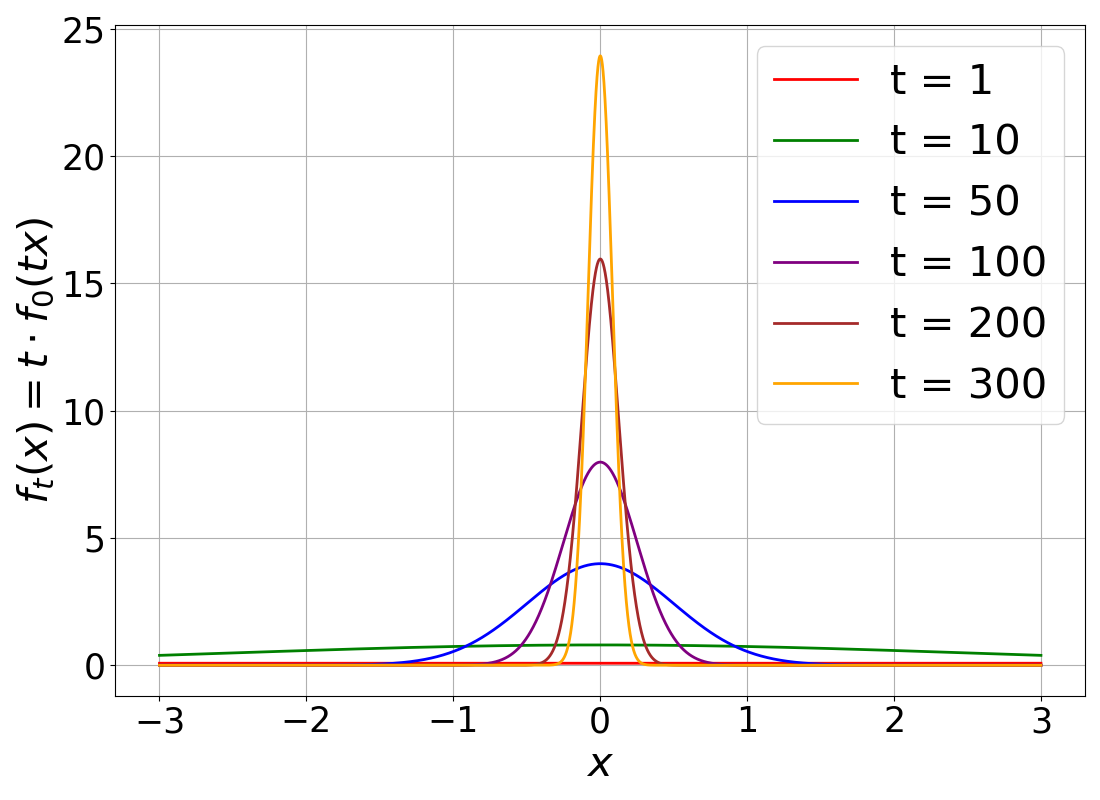
\includegraphics[width=0.97\textwidth]{fig/fig1_Normal.png}
        \vspace{-2mm}
        \caption{\footnotesize{Пример использования Теоремы \ref{delta} с $\psi_t = t$ для $\mathcal{N}(0; 1)$.}}
    \end{figure}
    \end{columns}
\end{frame}
%----------------------------------------------------------------------------------------------------------
\begin{frame}{Анализ условий существования петель обратной связи и автономности системы \eqref{system}}
\begin{columns}[c]
\column{0.55\textwidth}
    \begin{lemma_rus}[Стремление моментов к нулю] \label{moments}
        Если система \eqref{system} с $n=1$ удовлетворяет условиям Теоремы~\ref{delta} и $\psi_t \to \infty$, тогда все $2k$-тые моменты невязок 
        $y - h(X)$ убывают со скоростью как минимум $\psi_t^{-2k}$.
    \end{lemma_rus}
    \begin{figure}
        \centering
        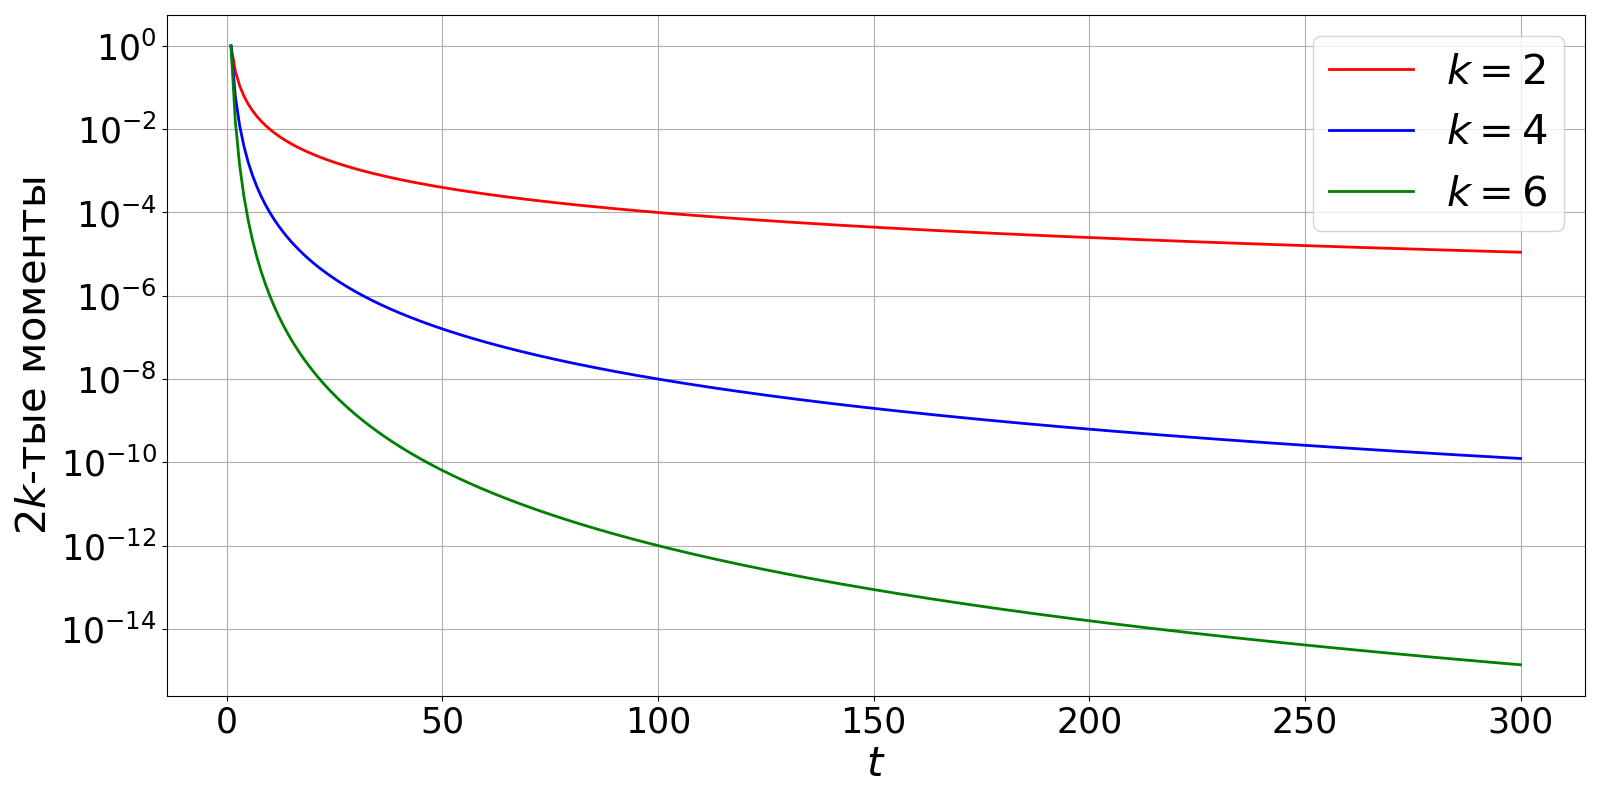
\includegraphics[width=0.9\textwidth]{fig/fig2.png}
        \vspace{-2mm}
        \caption{\footnotesize{Пример использования Леммы \ref{moments}.}}
    \end{figure}
\column{0.55\textwidth}
    \vspace{-4mm}
    \begin{theorem_rus}[Критерий автономности] \label{semigroup}
        Если операторы эволюции $\text{D}_t$ динамической системы \eqref{system} имеют вид $\text{D}_{\overline{1, t}}(f_0)(x) = \psi_t^n \cdot f_0(\psi_t \cdot x)$, тогда система \eqref{system} автономна тогда и только когда, когда $
            \psi_{\tau + \kappa} = \psi_{\tau} \cdot \psi_{\kappa} ~\forall \tau, \kappa \in \mathbb{N}.
        $
    \end{theorem_rus}
    \vspace{-2mm}
    \begin{figure}
        \centering
        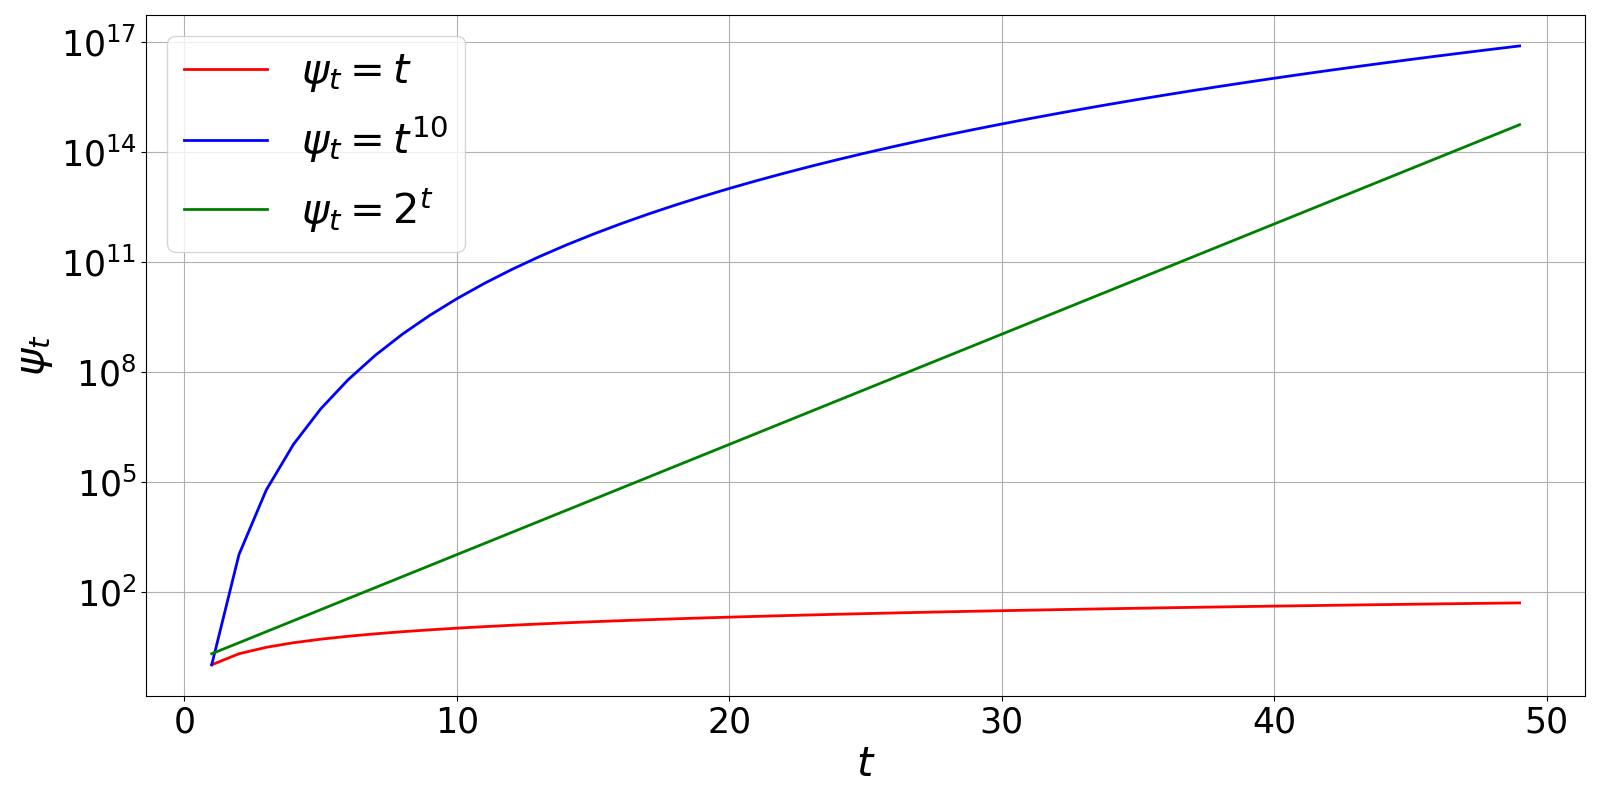
\includegraphics[width=0.95\textwidth]{fig/fig3.png}
        \vspace{-4mm}
        \caption{\footnotesize{Пример использования Теоремы \ref{semigroup}.}}
    \end{figure}
\end{columns}
\end{frame}
%----------------------------------------------------------------------------------------------------------
\begin{frame}{Предел к дельта-функции или нулевому распределению}
    \footnotesize
    \vspace{-2mm}
        \begin{figure}
            \centering
            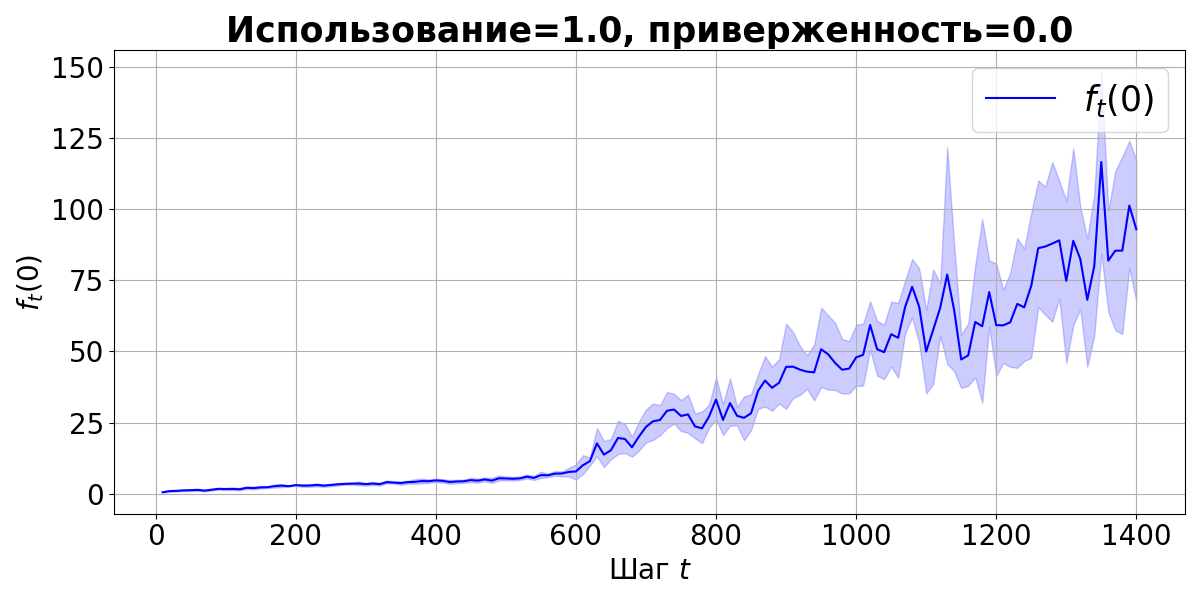
\includegraphics[width=0.49\linewidth]{fig/ft0_sw_synthetic_sgd_model_50_1.0_0.0.png}~
            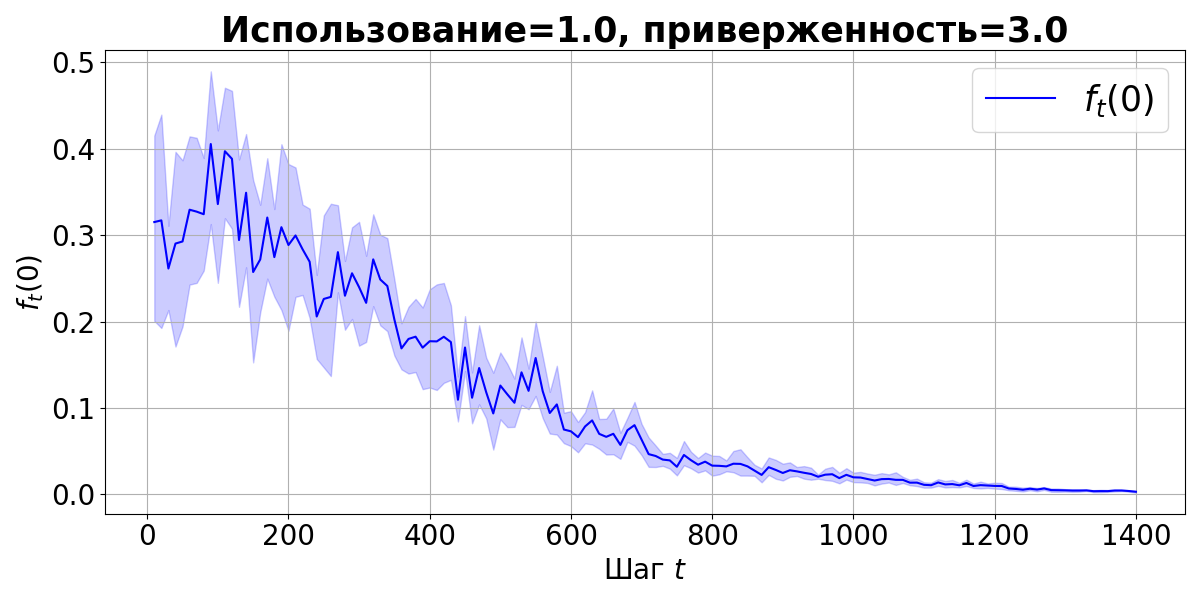
\includegraphics[width=0.49\linewidth]{fig/ft0_sw_synthetic_sgd_model_50_1.0_3.0.png}

            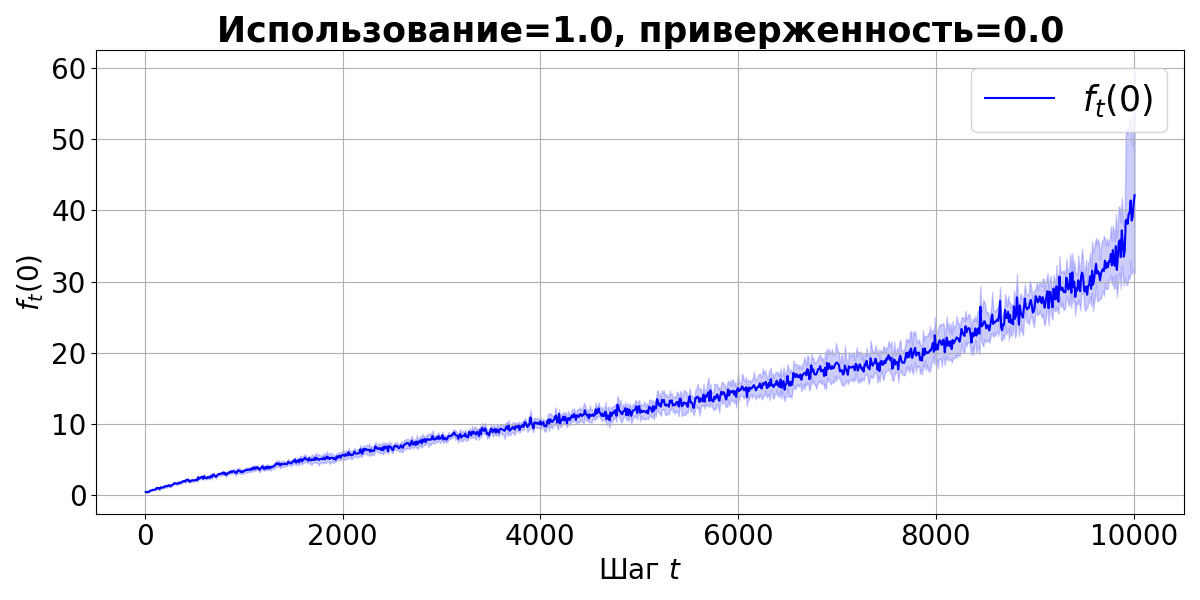
\includegraphics[width=0.49\linewidth]{fig/ft0_su_synthetic_sgd_model_50_1.0_0.0.png}~
            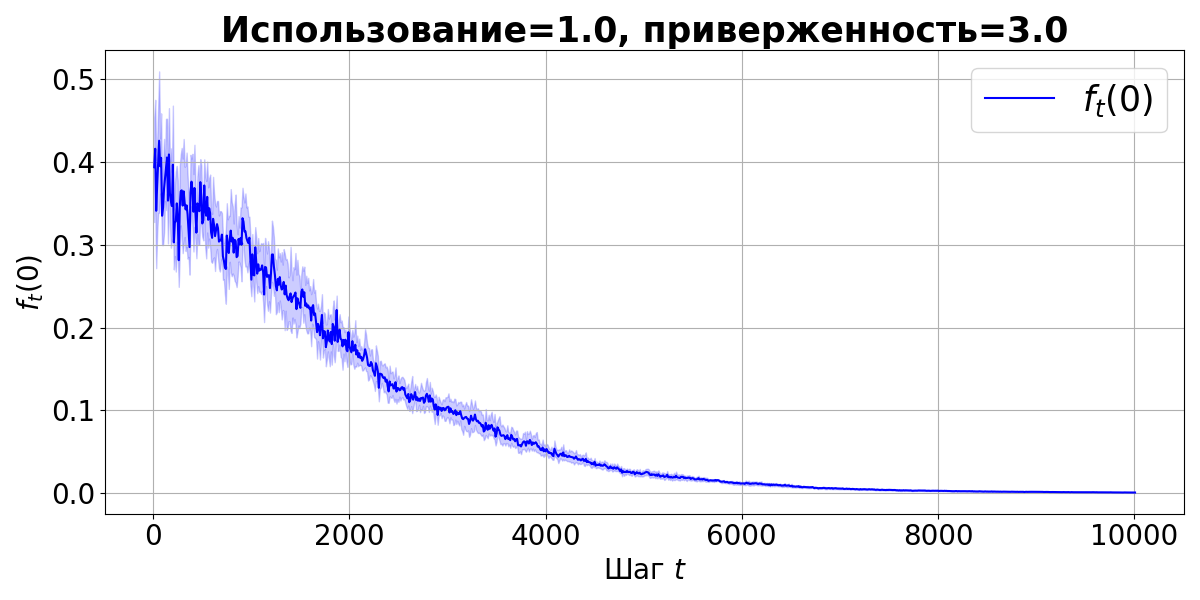
\includegraphics[width=0.49\linewidth]{fig/ft0_su_synthetic_sgd_model_50_1.0_3.0.png}
            \vspace{-4mm}
            \caption{Постановка скользящее окно (сверху), обновление выборки (снизу).}
        \end{figure}
    \end{frame}

    \begin{frame}{Стремление моментов к нулю и исследование систем на автономность}
    \footnotesize
    \vspace{-2mm}
        \begin{figure}
            \centering
            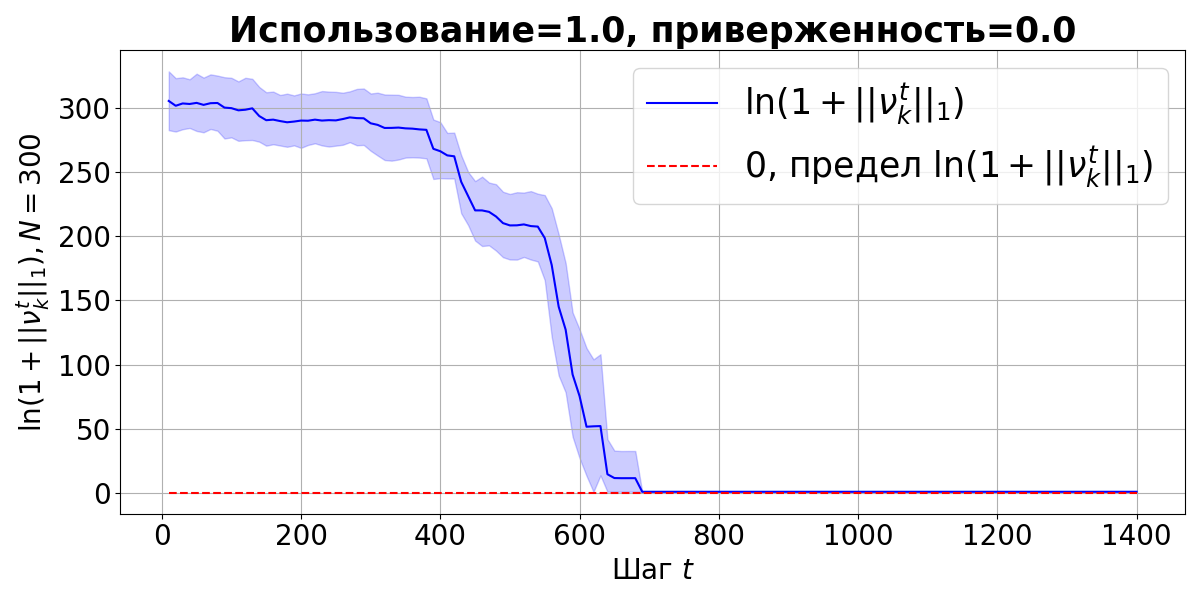
\includegraphics[width=0.49\linewidth]{fig/k_mom_sw_synthetic_sgd_model_50_1.0_0.0.png}~
            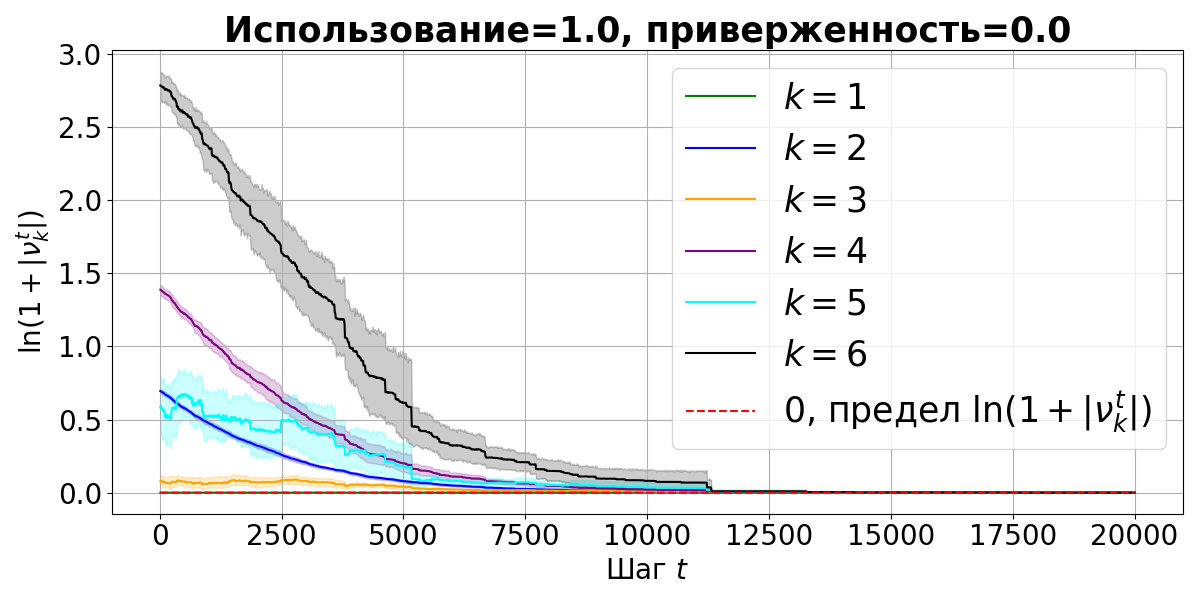
\includegraphics[width=0.49\linewidth]{fig/k_mom_su_synthetic_sgd_model_50_1.0_0.0.png}
            
            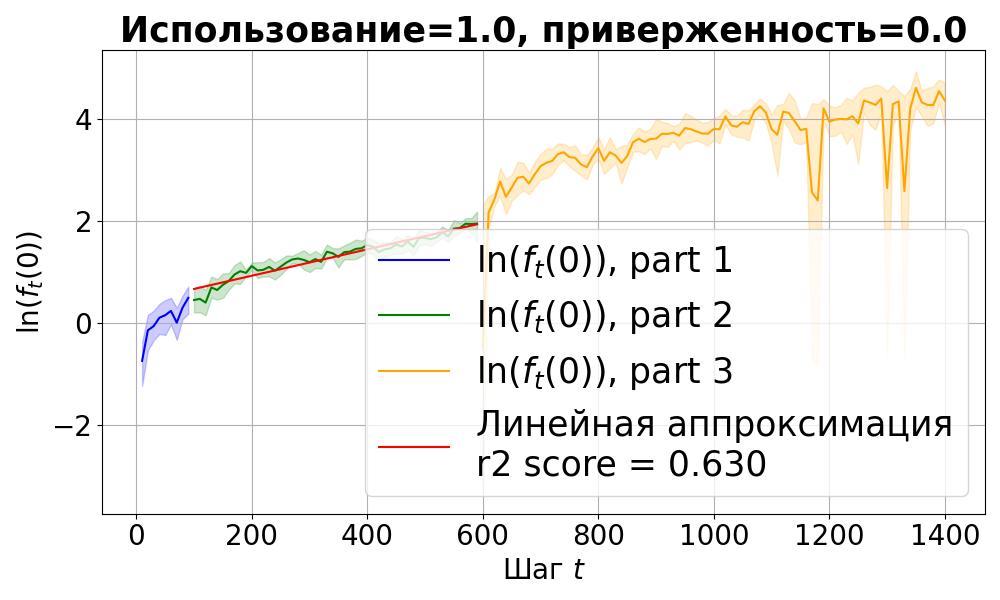
\includegraphics[width=0.326\linewidth]{fig/aut_sw_synthetic_sgd_model_50_1.0_0.0.png}
            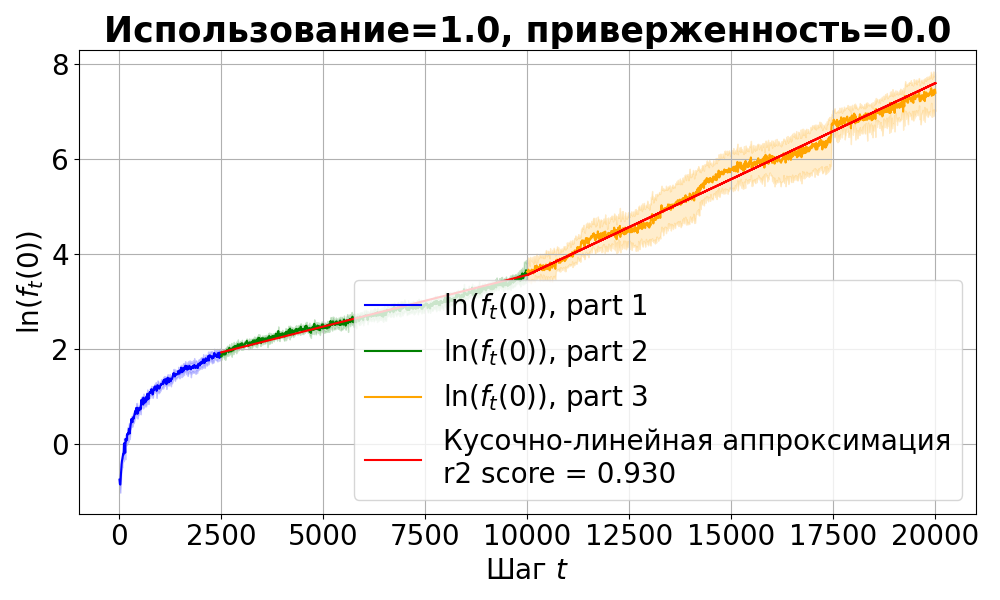
\includegraphics[width=0.326\linewidth]{fig/aut_su_synthetic_sgd_model_50_1.0_0.0.png}
            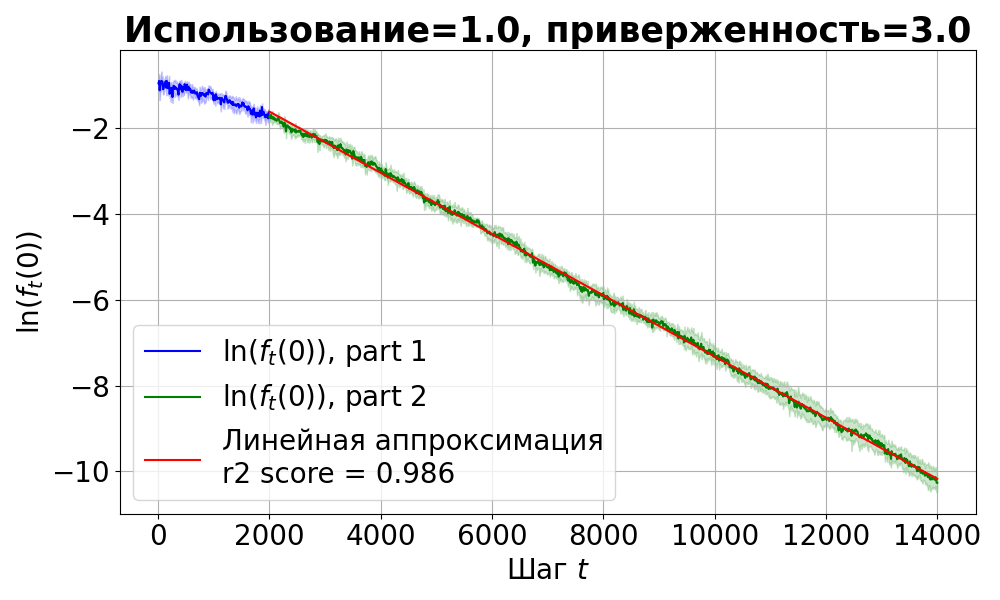
\includegraphics[width=0.326\linewidth]{fig/aut_su_synthetic_sgd_model_50_1.0_3.0.png}
            \vspace{-2mm}
            \caption{Стремление моментов к нулю(сверху): скользящее окно(слева), обновление выборки(справа).
            \centering{Проверка автономности(снизу): скользящее окно(слева), обновление выборки(середина и справа).}}
        \end{figure}
    \end{frame}
%----------------------------------------------------------------------------------------------------------
\begin{frame}{Выносится на защиту}
    \begin{enumerate}
        \item Построена математическая модель эффекта петель обратной связи с использованием дискретных динамических систем
        \item Были получены результаты для определения предельного множества динамической системы, достаточных условий существования петли обратной связи и критерий автономности
        \item Разработан стенд проведения вычислительных экспериментов, симулирующий процесс многократного машинного обучения
    \end{enumerate}
    \begin{block}{Публикации}%автора
    \footnotesize 
    \begin{enumerate}
        \item Veprikov A.,   Afanasiev A., Khritankov A. A Mathematical Model of the Hidden Feedback Loop Effect in Machine Learning Systems // arXiv preprint \url{https://arxiv.org/abs/2405.02726}
        \item Веприков А. С., Афанасьев А. П., Хританков А.С. Математическая модель эффекта обратной связи в системах искусственного интеллекта // Сборник тезисов 21-й Всероссийской конференции Математические методы распознавания образов (ММРО-21). – Российская академия наук, 2023. – С. 35-37 
    \end{enumerate}
    \end{block}
\end{frame}
%----------------------------------------------------------------------------------------------------------
\end{document} 